\documentclass{ferseminar}

\usepackage[table,xcdraw]{xcolor}
\usepackage{graphicx}
\usepackage{tikz}

\usetikzlibrary{tikzmark}
\tikzset{every picture/.style=remember picture}
\usetikzlibrary{matrix,fit}

\student{Antonio Benc, Matija Herceg, Luka Skukan}
\voditelj{doc. dr. sc. Mirjana Domazet-Lošo}
\mjestodatum{Zagreb}{siječanj}{2016}
\naslov{Algoritam za ažuriranje Burrows-Wheelerove transformacije u četiri koraka}

\setlength{\footskip}{20pt}
\begin{document}
\stvoripredstranice
\section{Uvod}
Burrows-Wheelerova transformacija (BWT) je transformacija teksta, vrlo prikladna za kompresiju. Njena primjena tipično rezultira poretkom u kojem isti znakovi često završavaju djelomično grupiranima. Nadalje, reverzibilna je bez potrebe za pohranom dodatnih podataka. Stoga se koristi u nekim popularnim alatima za kompresiju bez gubitaka, primjerice programu bzip2.  Osim pod nazivom Burrows-Wheelerova transformacija, poznata je i pod nazivom \textit{block-sorting compression}. 


Konceptualno, tekst nad kojim je izvršena BWT je sličan sufiksnom polju. Zbog te sličnosti BWT se koristi i kao indeksna struktura. BWT tseksta $T$ ($bwt(t)$) se često dobiva iz modifikacije sufiksnog polja složenost čije konstrukcije je $O(n)$. Pohranjivanje sufiksnog polja u memoriji još je uvijek glavni problem jer zahtjeva $n\log{}n$ bitova, dok pohrana BWT-a u memoriju zahtjeva tek $(n\log{}\sigma)$ bita, gdje je $\sigma$ broj simbola u korištenoj abecedi $\Sigma$.


U ovom seminaru razmatrat će se uobičajene operacije nad tekstom - umetanje znakova, brisanje znakova ili zamjena znakova, koje tekst $T$ transformiraju u novi tekst $T'$. Biti će proučavan utjecaj tih operacija na $bwt(T)$ i biti će opisane operacije pretvorbe $bwt(T)$ u $bwt(T')$, te njihova implementacija.

\section{Burrows-Wheelerova transformacija}

Neka je tekst $T=T[0..n]$ riječ duljine $n+1$ s abecedom $\Sigma$, pri čemu je abeceda $\Sigma$ konačne veli;ine $\sigma$. Zadnji znak u riječi $T$ je jedinstveni znak $\$$ (\textit{sentinel}) koji ima vrijednost manju od svih ostalih znakova u abecedi, odnosno pri operaciji usporedbe uvijek se smatra manjim.  Podniz koji počinje na poziciji $i$ i završava na poziciji $j$ označen je s $T[i..j]$, znak na poziciji $i$ je označen s $T[i]$, te je ciklički pomak reda $i$,  $T[i..n]T[0..i-1]$ označen s $T^{[i]}$.

Burrows-Wheelerova transformacija od $T$, označena s $bwt(T)$, je tekst duljine n+1 koji odgovara zadnjem stupcu, ($L$), matrice čiji su reci leksikografski sortirani ciklički pomaci $T^{[i]}$. Prvi stupac matrice, ($F$), je sortiran, tako da se jednostavno može izračunati iz stupca $L$. Redovi sortiranih cikličkih pomaka, $\pi$ jednaki su sufiksnom polju od $T$. Iz toga slijedi kako su sufiksno polje $SA[i]$ i $L$ povezani jednostavnom formulom $L[i]= T[(SA[i]-1) \mod |T|]$.

\begin{table}[h]

\begin{tabular}{r c c c c c c c c c r c c c c c c c c c c}
		
		  &   &  &  &  &  &  	
      & & & & & & & & 
      & & & \multicolumn{1}{l|}{i} & $\pi$    \\ 
	  \cline{2-7} \cline{11-16} \cline{18-19}
      \multicolumn{1}{l|}{$T^{[0]}$} & A & T & G & C & G & \multicolumn{1}{l|}{\$} &  	
      & &    \multicolumn{1}{l|}{$T^{[5]}$} & \$ & A & T & G & C & \cellcolor[HTML]{9B9B9B} G
      & & \multicolumn{1}{l|}{0} & 5    \\ 
      
	 \multicolumn{1}{l|}{$T^{[1]}$} & T & G & C & G & \$ & \multicolumn{1}{l|}{A} &
	  & &    \multicolumn{1}{l|}{$T^{[0]}$} & A & T & G & C & G & \cellcolor[HTML]{9B9B9B} \$
	  & & \multicolumn{1}{l|}{1} & 0     \\ 
	  
	  \multicolumn{1}{l|}{$T^{[2]}$} & G & C & G & \$ & A & \multicolumn{1}{l|}{T} & 
	  & &    \multicolumn{1}{l|}{$T^{[3]}$} & C & G & \$ & A & T & \cellcolor[HTML]{9B9B9B} G
	  & & \multicolumn{1}{l|}{2} & 3     \\ 
	  
	  \multicolumn{1}{l|}{$T^{[3]}$} & C & G & \$ & A & T & \multicolumn{1}{l|}{G} & $\Rightarrow$
	  & &    \multicolumn{1}{l|}{$T^{[4]}$} & G & \$ & A & T & G & \cellcolor[HTML]{9B9B9B} C
	  & $\Rightarrow$ & \multicolumn{1}{l|}{3} & 4     \\ 
	  
	  \multicolumn{1}{l|}{$T^{[4]}$} & G & \$ & A & T & G & \multicolumn{1}{l|}{C} & 
	  & &   \multicolumn{1}{l|}{$T^{[2]}$} & G & C & G & \$ & A & \cellcolor[HTML]{9B9B9B} T
	  & & \multicolumn{1}{l|}{4} & 2     \\
	  
	  \multicolumn{1}{l|}{$T^{[5]}$} & \$ & A & T & G & C & \multicolumn{1}{l|}{G} &	
	  & &    \multicolumn{1}{l|}{$T^{[1]}$} & T & G & C & G & \$ & \cellcolor[HTML]{9B9B9B} A
	  & & \multicolumn{1}{l|}{5} & 1     \\
	  
	   \cline{2-7} \cline{11-16}
	  			&	 &	 &	 &	 & 	 &					& & &			  &$F$&	  &	  &	  & & $L$	  \\
 
\end{tabular}
\caption{Burrows-Wheelerova transformacija niza $ATGCG\$$}
\label{tablica:bwt}	
\end{table}

Tablicom \ref{tablica:bwt} prikazana je Burrows-Wheelerova transformacija niza znakova $ATGCG\$$. U lijevoj prikazani su svi ciklički pomaci tog niza. U središnjoj tablici, ti su ciklički pomaci leksikografski sortirani i označeni su stupci $F$ i $L$, odnosno prvi i zadnji stupac. U desnoj tablici prikazan je niz brojeva koji predstavljaju  indekse redova sortiranih cikličkih pomaka, ujedno i sufiksno polje od niza.

Burrows-Wheelerova transformacija odgovara zadnjem stupcu sortirane matrice cikličkih pomaka, odnosno $L$. Za rekonstrukciju početnog niza niza $T$ iz $bwt(t)$ koristi se veza između stupca L i stupca F. Ako znakovima u primjeru s $ATGCG\$$ svakom znaku pridjelimo broj koji označava redni broj pojavljivanja tog slova u tekstu $T$, dobivamo niz $A_{1}T_{1}G_{1}C_{1}G_{2}\$_{1}$.

\begin{table}[h]
\begin{center}


\begin{tabular}{r c c c c c c}
	\multicolumn{1}{l|}{$T^{[5]}$} & $\$_{1}$ & $A_{1}$ & $T_{1}$ & $G_{1}$ & $C_{1}$ & \cellcolor[HTML]{9B9B9B} $G_{2}$ \\
	\multicolumn{1}{l|}{$T^{[0]}$} & $A_{1}$ & $T_{1}$ & $G_{1}$ & $C_{1}$ & $G_{2}$ & \cellcolor[HTML]{9B9B9B} $\$_{0}$ \\
	\multicolumn{1}{l|}{$T^{[3]}$} & $C_{1}$ & $G_{2}$ & $\$_{1}$ & $A_{1}$ & $T_{1}$ & \cellcolor[HTML]{9B9B9B} $G_{1}$ \\
	\multicolumn{1}{l|}{$T^{[4]}$} & $G_{2}$ & $\$_{1}$ & $A_{1}$ & $T_{1}$ & $G_{1}$ & \cellcolor[HTML]{9B9B9B} $C_{1}$ \\
	\multicolumn{1}{l|}{$T^{[2]}$} & $G_{1}$ & $C_{1}$ & $G_{2}$ & $\$_{1}$ & $A_{1}$ & \cellcolor[HTML]{9B9B9B} $T_{1}$ \\
	\multicolumn{1}{l|}{$T^{[1]}$} & $T_{1}$ & $G_{1}$ & $C_{1}$ & $G_{2}$ & $\$_{1}$ & \cellcolor[HTML]{9B9B9B} $A_{1}$ \\ 
\end{tabular}
\caption{Burrows-Wheelerova transformacija niza $ATGCG\$$ s rangiranim znakovima}
\label{tablica:ibwt}	
\end{center}
\end{table}

Tablicom \ref{tablica:ibwt} prikazani su rangirani ciklični pomaci s rangiranim znakovima zajedno sa stupcima $L$ i $F$. Rotacije koje počinju istim slovom, u primjeru slovom G, sortirane su po znakovima koji slijede. Kada se te rotacije ciklički rotiraju za jedno mjesto, slova G će se naći u zadnjem stupcu, dok druga slova biti na početku niza i određivati će leksikografski poredak tih rotacija. Upravo zato je redoslijed istih slova u prvom stupcu jednak redoslijedu istih slova u zadnjem stupcu. Ovo svojstvo očuvanosti poretka istih znakova u prvom i zadnjem stupcu BWT-a naziva se LF-mapiranje (last to first mapping) i omogućuje rekonstrukciju početnog niza iz BWT-a. Formalnije, LF-mapiranje opisuje vezu, odnosno mapiranje, zadnjeg i prvog stupca u listi leksikografski sortiranih cikličkih rotacija niza S, a temelji se na sljedećem: $i$-ta pojava znaka $c$ u zadnjem stupcu (stupcu $L$) leksikografski sortiranih cikličkih rotacija
odgovara $i$-toj pojavi znaka $c$ u prvom stupcu (stupcu $F$). LF mapiranjem, iz BWT-a i uz prisutnost stupca $L$, moguće je izgraditi početni niz. Stupac F može se dobiti tako da se leksikografski poredaju svi znakovi u stupcu $L$, odnosno BWT-u.

Formula za LF mapiranje znaka na poziciji $p$ glasi:
\begin{equation}
	LF(p)=C_T[L[p]]+rank_{L[p]}(L,p)-1 ,
\end{equation}

gdje je $C_T$ broj znakova u nizu manjih od znaka $L[p]$, $rank_{L[p]}(L,p)$ broj pojavljivanja znaka $L[p]$ u $L$ do pozicije $p$.

Stupac $L$, odnosno BWT je konceptualno blizak sufiksnom polju, a povezuje ih jednostavna transformacija. Stoga se većina algoritama za konstrukciju BWT-a bazira na postojećim algoritmima za računanje sufiksnog polja s kompleksnošću $O(n)$ i primjeni transformacije sufiksnog polja u BWT.

Jednostavna transformacija niza $T$ u niz $T'$ uzrokuje da se BWT od $T'$ mora računati od nule. U nastavku seminara biti će proučeno kako jednostavne operacije nad nizom $T$ utječu na $bwt(T)$. 

\section{Opis algoritma}
Opis će biti temeljen na slučaju kada se u niz umeće samo jedan znak. Na temelju toga biti će predstavljen algoritam u četiri koraka za ažuriranje BWT-a. Kako bi se mogao ažurirati BWT, potrebno je i ažurirati parcijalne sume (gore objasniti parcijalne sume znakova). Zatim će se taj pristup proširiti na više znakova i na zamjenu i brisanje znakova.

BWT je usko povezan s leksičkim sortiranjem svih cikličkih pomaka niza $T'$. Pretpostavka je da se u niz $T$ umeće slovo $c$ na poziciju $i$. Prema tome, postoje 4 slučaja koji su opisani slikom \ref{tablica:pozicije}. 

\begin{figure}[h]
\scriptsize
\[ 
T'^{[j]}=\left \{
  \begin{tabular}{rcllc}
  $T[j-i\ .. \ n-1]$ & $\$$ & $T[0 \ .. \ i-1]\quad c\quad  T[i \ .. \ j-2]$ & ako je $i+1<j\leq n+1$ & (Ia)\\
  $T[i \ .. \ n-1]$ & $\$$  & $T[0 \ .. \ i-1] \quad c$ & ako je $j= n+1$ & (Ib)\\
  $c \quad T[i \ .. \ n-1]$ & $\$$  & $T[0 \ .. \ i-1] \quad$ & ako je $j=1$ & (IIa)\\
  $T[j \ .. \ i-1] \quad c \quad T[i \ .. \ n-1]$ & $\$$  & $T[0 \ .. \ j-1]$ & ako je $0 \leq j< 1$ & (IIb)\\
  
  \end{tabular}
\right.
\]
\small
\begin{tabular}{ccccccc}
 \cline{1-3} \cline{5-7}
 \multicolumn{3}{|c|}{(II)\tikzmark{II}} & $\$$ & \multicolumn{3}{|c|}{(I)\tikzmark{I} }\\
 \cline{1-3} \cline{5-7}
  & & & & & & \\
  \cline{1-1}  \cline{3-3} \cline{5-5} \cline{7-7}
  \multicolumn{1}{|c|}{(IIa)\tikzmark{IIa}}& & \multicolumn{1}{|c|}{$\qquad$(IIb)\tikzmark{IIb}$\qquad$} & $\$$ &\multicolumn{1}{|c|}{$\qquad$(Ia)\tikzmark{Ia}$\qquad$} & & \multicolumn{1}{|c|}{(Ib)\tikzmark{Ib}} \\
   \cline{1-1}  \cline{3-3} \cline{5-5} \cline{7-7}
  
 

\end{tabular}
\begin{tikzpicture}[overlay, remember picture, yshift=.25\baselineskip, shorten >=.5pt, shorten <=.5pt]
    \draw [->] ([xshift=-6pt,yshift=-8pt]{pic cs:II})  to ([xshift=-6pt,yshift=8pt]{pic cs:IIa});
    \draw [->] ([xshift=-6pt,yshift=-8pt]{pic cs:II})  to ([xshift=-8pt,yshift=8pt]{pic cs:IIb});
    
    \draw [->] ([xshift=-6pt,yshift=-8pt]{pic cs:I})  to ([xshift=-8pt,yshift=8pt]{pic cs:Ia});
    \draw [->] ([xshift=-6pt,yshift=-8pt]{pic cs:I})  to ([xshift=-8pt,yshift=8pt]{pic cs:Ib});
    
\end{tikzpicture}


\caption{Moguće pozicije znaka $c$ u cikličkim rotacijama}
\label{tablica:pozicije}
\end{figure}
\normalsize

\subsection{Ciklički pomaci reda $j>i$ (I)}
Pozicija umetanja znaka $i$ u ovom slučaju je manja od reda rotacije cikličkog pomaka $j$, što znači da će se u cikličkom pomaku umetnuti znak nalazi iza znaka $\$$ kao što je prikazano na slici\ref{tablica:pozicije}. Pokazuje se da u ovom slučaju poredak cikličkih pomaka ne mijenja. 

\subsubsection{Ciklički pomaci reda $j>i+1$ (Ia)}
U ovom slučaju znak $c$ se dodaje između znaka $\$$ i zadnjeg stupca $L$, tako da su stupci $F$ i $L$ nepromijenjeni.

\subsubsection{Ciklički pomaci reda $j=i+1$ (Ib)}
Poredak cikličkih pomaka je i u ovom slučaju isti. Iz slike \ref{tablica:pozicije} je vidljivo kako se c dodaje na kraj cikličkog pomaka što uzrokuje promjenu zadnjeg stupca $L$, $T'^{[i+1]}=T^[i]c$. Kako bi se provela ova modifikacija prvo je potrebno pronaći poziciju redka koji odgovara pomaku za $i$ i zamijeniti znak na tom mjestu u $c$. Poziciju retka koji odgovara pomaku  $i$ moguće je pronaći korištenjem uzorkovanog sufiksnog polja i pozicije $k$ takve da je $k=SA[i]$. Pomak $T^{[i]}$ može biti preskočen kod uzorkovanja tako da je potrebno koristiti sljedeću otipkanu poziciju koja odgovara cikličkom pomaku $T^{[j]}$. Red $j$ je takav da je $j>i$ i takav da ne postoji pomak $T^{[j']}$ za koji vrijedi $i<j'<j$. LF mapiranje omogućava da se preko cikličkog pomaka reda $j$ dođe do cikličkog pomaka $j-1$, tako da se korištenjem LF funkcije $j-i$ puta može doći do cikličkog pomaka $T^{[i]}$. Konačno, moguće je zamijeniti slovo u L stupcu, $L[k]=c$, gdje sada element u stupcu $L$ na poziciji $k$ odgovara pomaku $T'^{[i+1]}$.
U nastavku su prikazani koraci (Ia) i (Ib) na primjeru.

\begin{minipage}{0.5\textwidth}
\footnotesize
Umetanje znaka G na poziciju $i=2$ u $T$
$$
	T=\overset{0}{C}	\overset{1}{T} \overset{2}{C} \overset{3}{T}	\overset{4}{G}
	\overset{5}{C}	\overset{6}{\$} \rightarrow		
	T'=\overset{0}{C}	\overset{1}{T}	\overset{2}{\boldsymbol{G}}  \overset{3}{C} \overset{4}{T}	\overset{5}{G}
	\overset{6}{C}	\overset{7}{\$} 	
$$
\begin{itemize}
  \item[(Ia)] Nema modifikacije.
  \item[(Ib)] $T^{[i]}$ je na poziciji $k=3$ ($SA[3]=\pi(3)=2$), $L[3]\leftarrow \boldsymbol{G}$.
\end{itemize}
\end{minipage} \hfill
\begin{minipage}{0.45\textwidth}
\begin{tabular}{cccc|ccc|cc}
	& $\pi$ &  & F & L & & F & L \\
	\cline{2-2} \cline{4-5} \cline{7-8}
	& 6 & & \$ & C & & \$ & C \\
	& 5 & & C & G & & C & G \\
	& 0 & & C & \$ & & C & \$ \\
	\cline{1-8}
	\multicolumn{1}{|c}{$i=$}& 2 & & C & T & $\stackrel{(Ib)}{\longrightarrow}$ & C & \multicolumn{1}{c|}{G} \\
	\cline{1-8}
	& 4 & & G & T & & G & T \\
	& 1 & & T & C & & T & C \\
	& 3 & & T & C & & T & C 
\end{tabular}

\end{minipage}


\subsection{Ciklički pomaci reda $j\leq i$ (II)}

\subsubsection{Ciklički pomaci reda $j=i$ (IIa)}
Nakon razmatranja cikličkog pomaka $T'^{[i+1]}$ koji završava s dodanim znakom $c$, razmatra se potpuno novi ciklički pomak koji počinje s $c$, $T'^{[i]}=cT^{[i]}=cT[i..n-1]\$T[0..i-1]$, kao što je prikazani slikom \ref{tablica:pozicije}. Budući da je $T'^{[i+1]}$ na prethodno izračunatoj poziciji k, $T'^[i]$ mora biti umetnut na poziciju $LF(k)$.

\begin{minipage}{0.5\textwidth}
\footnotesize
Umetanje znaka G na poziciju $i=2$ u $T$
$$
	T=\overset{0}{C}	\overset{1}{T} \overset{2}{C} \overset{3}{T}	\overset{4}{G}
	\overset{5}{C}	\overset{6}{\$} \rightarrow		
	T'=\overset{0}{C}	\overset{1}{T}	\overset{2}{\boldsymbol{G}}  \overset{3}{C} \overset{4}{T}	\overset{5}{G}
	\overset{6}{C}	\overset{7}{\$} 	
$$
\begin{itemize}
  \item[] (IIa): $T'^{[i]}$ je umetnut na poziciju $LF(k)$
  \item[] Za novo umetnuti pomak vrijedi $F=c=\boldsymbol{G}$ i $L=T_{i-1}=\boldsymbol{T}$.
  \item[] $T'^{[i-1]}$ završava s G koji je drugi G u $L$.
  \item[] $T'^{[i]}$ počinje s G koji mora biti drugi G u $F$.
\end{itemize}

\end{minipage} \hfill
\begin{minipage}{0.45\textwidth}
\hspace{.2\textwidth}
\begin{tabular}{cccc|cc}
	\multicolumn{1}{c|}{F} & L & & F & L \\
	\cline{1-2}	\cline{4-5}
	\multicolumn{1}{c|}{\$} & C & & \$ & C \\
	\multicolumn{1}{c|}{C} & G & & C & G \\
	\multicolumn{1}{c|}{C} & \$ & & C & \$ \\
	
	\multicolumn{1}{c|}{C} & $\boldsymbol{G}$ & $\stackrel{(IIa)}{\longrightarrow}$ & C & G \\
	
	\multicolumn{1}{c|}{G} & T & & G & T \\
	\cline{4-5}
	\multicolumn{1}{c|}{T} & C & & \multicolumn{1}{|c|}{$\boldsymbol{G}$} & \multicolumn{1}{c|}{$\boldsymbol{T}$} \\
	\cline{4-5}
	\multicolumn{1}{c|}{T} & C & & T & C \\
	  &   & & T & C
\end{tabular}

\end{minipage}

\subsubsection{Ciklički pomaci reda $j<i$ (IIb)}
U prethodnim koracima, vrijednost u jednom elementu stupca $L$ je bila izmijenjena (Ib) i jedan element je dodan (IIa). No u slučaju $j<i$, ciklički pomaci $T'^[j]$ mogu imati drugačiji leksikografski poredak od $T^{[j]}$, zbog čega neki reci moraju biti pomaknuti.

Kako bi se ustanovilo koji reci moraju biti pomaknuti, uspoređuju se pozicije $T^{[j]}$ s pozicijama $T'^{[j]}$, od $j=i-1$ pa do $0$, dok pozicije nisu jednake. Pozicija $T^{[j]}$ dobiva se pomoću LF mapiranja iz pozicije $T^{[j+1]}$. Isto tako pozicija pozicija $T'^{[j]}$ dobiva se pomoću LF mapiranja iz pozicije $T'^{[j+1]}$. Kada se te dvije pozicije razlikuju, redak koji odgovara $T^{[j]}$ miče se na izračunatu poziciju $T'^{[j]}$. Pokazuje se da su nakon što su te dvije pozicije jednake reci ispravno poredani.
U nastavku je prikazan pseudokod za korak (IIb). Funkcija indeks vraća poziciju cikličkog pomaka.

\footnotesize
\begin{enumerate}
	\item $j\longleftarrow index(T^{[i-1]}) \quad$ $\triangleright$ Daje poziciju $T^{[i-1]}$
	\item $j'\longleftarrow LF(index(T'^{[i-1]})) \quad$ $\triangleright$ Daje izračunatu poziciju $T'^{[i-1]}$
	\item \textbf{dok je} $j\neq j'$
	\item \hspace{.1\textwidth} $novi\_j \longleftarrow LF(j) $
	\item \hspace{.1\textwidth} $pomakniRedak(L,j,j')$
	\item \hspace{.1\textwidth} $j \longleftarrow novi\_j $
	\item \hspace{.1\textwidth} $j' \longleftarrow LF(j') $
\end{enumerate}
\normalsize
Za primjer korišten za demonstraciju prethodnih koraka, $
	T=\overset{0}{C}	\overset{1}{T} \overset{2}{C} \overset{3}{T}	\overset{4}{G}
	\overset{5}{C}	\overset{6}{\$} \rightarrow		
	T'=\overset{0}{C}	\overset{1}{T}	\overset{2}{\boldsymbol{G}}  \overset{3}{C} \overset{4}{T}	\overset{5}{G}
	\overset{6}{C}	\overset{7}{\$} 	
$, u tablici \ref{slika:korak2b} prikazan je korak (IIb). Kreće se od pomaka $T^{[i-1]}$. On je na poziciji s indeksom 6. LF od $T'^{[i]}$ (na poziciji s indeksom 5) iznosi $LF=C_T(T)+rank_T(L,5)-1=7$. Pozicije nisu iste, pa je pomak $T^{[i-1]}$ potrebno pomaknuti na poziciju s indeksom 7.

Dalje slijedi pomak $T^{[i-1]}$, koji je na poziciji s indeksom 2. LF od $T'^{[i-1]}$, koji je na poziciji s indeksom 7, iznosi $LF=C_T(C)+rank_T(L,7)-1=3$. Pozicije su opet različiti, pa pomak $T^{[i-1]}$ treba premjestiti na poziciju 3.

Na poziciji $T'^{[i-2]}$ je prvi $\$$ u $L$ i na poziciji $T^{[i-3]}$ je prvi $\$$ u $F$ iz čega se može zaključiti kako više nije potrebno pomicati cikličke pomake. Uz to dosegnuta je i pozicija 0 koja označava kraj koraka. 

\begin{figure}[!h]
\label{slika:korak2b}
\scriptsize
\centering
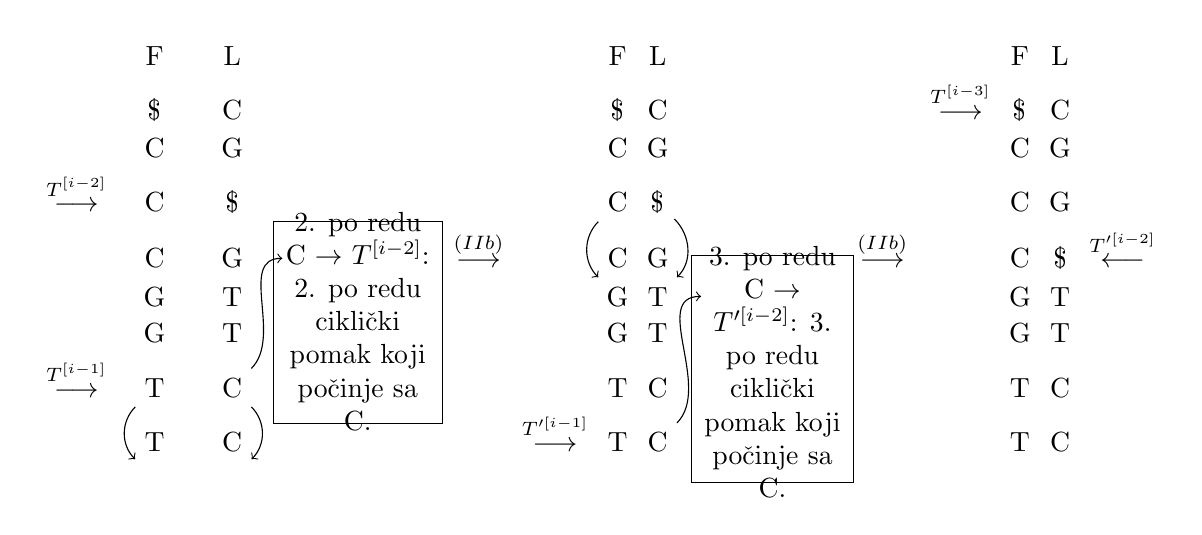
\begin{tikzpicture}
\matrix [matrix of nodes,row sep=-\pgflinewidth,name=table,column 4/.style={nodes={,minimum width=1.9cm}},column 9/.style={nodes={,minimum width=1.8cm}}](m)
{
	& F & L & [1ex] & [1ex] & & F & L & [2ex] & & & F & L & \\
	& \$ & C & & & & \$ & C & & & $\stackrel{T^{[i-3]}}{\longrightarrow}$ & \$ & C & \\
	& C & G & & & & C & G & & & & C & G & \\
	$\stackrel{T^{[i-2]}}{\longrightarrow}$& C & \$ & & & & C & \$  & & & & C & G & \\
	& C & G & \phantom{dank} & $\stackrel{(IIb)}{\longrightarrow}$ & & C & G & &$\stackrel{(IIb)}{\longrightarrow}$ & & C & \$ & $\stackrel{T'^{[i-2]}}{\longleftarrow}$ \\
	& G & T &  & & & G & T & \phantom{dank} & & & G & T & \\
	& G & T &  & & & G & T & \phantom{dank} & & & G & T & \\
	$\stackrel{T^{[i-1]}}{\longrightarrow}$& T & C & \phantom{dank} & & & T & C & \phantom{dank} & \phantom{dank} & & T & C & \\
	& T & C & \phantom{dank} & & $\stackrel{T'^{[i-1]}}{\longrightarrow}$ & T & C & \phantom{dank} & & & T & C & \\
	& \phantom{dank} & \phantom{dank} &   & &  &  &    & & &  &  & \\
};
\draw[->] (m-8-2) to [out=-135,in=135] (m-10-2);
\draw[->] (m-8-3) to [out=-45,in=45] (m-10-3);

\node[draw,fit=(m-5-4)(m-8-4)]{2. po redu C $\rightarrow$ $T^{[i-2]}$: 2. po redu ciklički pomak koji počinje sa C. };
\node[draw,fit=(m-6-9)(m-9-9)]{3. po redu C $\rightarrow$ $T'^{[i-2]}$: 3. po redu ciklički pomak koji počinje sa C. };

\draw[->] (m-4-8) to [out=-45,in=45] (m-6-8);
\draw[->] (m-4-7) to [out=-135,in=135] (m-6-7);

\draw[->] (m-8-3) to [out=45,in=180] (m-5-4);
\draw[->] (m-9-8) to [out=45,in=180] (m-6-9);

\end{tikzpicture}
\end{figure}
\normalsize

\subsection{Ciklički pomaci reda $j\leq i$ (II)}
\subsubsection{Ciklički pomaci reda $j=i$ (IIa)}
Nakon razmatranja cikličkog pomaka $T'^{[i+1]}$ koji završava s dodanim znakom $c$, razmatra se potpuno novi ciklički pomak koji počinje s $c$, $T'^{[i]}=cT^{[i]}=cT[i..n-1]\$T[0..i-1]$, kao što je prikazani slikom \ref{tablica:pozicije}. Budući da je $T'^{[i+1]}$ na prethodno izračunatoj poziciji k, $T'^[i]$ mora biti umetnut na poziciju $LF(k)$. [ovdje nešto za korištenu strukturu i parcijalne sume]

\begin{minipage}{0.5\textwidth}
\footnotesize
Umetanje znaka G na poziciju $i=2$ u $T$
$$
	T=\overset{0}{C}	\overset{1}{T} \overset{2}{C} \overset{3}{T}	\overset{4}{G}
	\overset{5}{C}	\overset{6}{\$} \rightarrow		
	T'=\overset{0}{C}	\overset{1}{T}	\overset{2}{\boldsymbol{G}}  \overset{3}{C} \overset{4}{T}	\overset{5}{G}
	\overset{6}{C}	\overset{7}{\$} 	
$$
\begin{itemize}
  \item[] (IIa): $T'^{[i]}$ je umetnut na poziciju $LF(k)$
  \item[] Za novo umetnuti pomak vrijedi $F=c=\boldsymbol{G}$ i $L=T_{i-1}=\boldsymbol{T}$.
  \item[] $T'^{[i-1]}$ završava s G koji je drugi G u $L$.
  \item[] $T'^{[i]}$ počinje s G koji mora biti drugi G u $F$.
\end{itemize}

\end{minipage} \hfill
\begin{minipage}{0.45\textwidth}
\hspace{.2\textwidth}
\begin{tabular}{cccc|cc}
	\multicolumn{1}{c|}{F} & L & & F & L \\
	\cline{1-2}	\cline{4-5}
	\multicolumn{1}{c|}{\$} & C & & \$ & C \\
	\multicolumn{1}{c|}{C} & G & & C & G \\
	\multicolumn{1}{c|}{C} & \$ & & C & \$ \\
	
	\multicolumn{1}{c|}{C} & $\boldsymbol{G}$ & $\stackrel{(IIa)}{\longrightarrow}$ & C & G \\
	
	\multicolumn{1}{c|}{G} & T & & G & T \\
	\cline{4-5}
	\multicolumn{1}{c|}{T} & C & & \multicolumn{1}{|c|}{$\boldsymbol{G}$} & \multicolumn{1}{c|}{$\boldsymbol{T}$} \\
	\cline{4-5}
	\multicolumn{1}{c|}{T} & C & & T & C \\
	  &   & & T & C
\end{tabular}

\end{minipage}




\subsubsection{Ciklički pomaci reda $j<i$ (IIb)}
U prethodnim koracima, vrijednost u jednom elementu stupca $L$ je bila izmijenjena (Ib) i jedan element je dodan (IIa). No u slučaju $j<i$, ciklički pomaci $T'^[j]$ mogu imati drugačiji leksikografski poredak od $T^{[j]}$, zbog čega neki reci moraju biti pomaknuti.

Kako bi se ustanovilo koji reci moraju biti pomaknuti, uspoređuju se pozicije $T^{[j]}$ s pozicijama $T'^{[j]}$, od $j=i-1$ pa do $0$, dok pozicije nisu jednake. Pozicija $T^{[j]}$ dobiva se pomoću LF mapiranja iz pozicije $T^{[j+1]}$. Isto tako pozicija pozicija $T'^{[j]}$ dobiva se pomoću LF mapiranja iz pozicije $T'^{[j+1]}$. Kada se te dvije pozicije razlikuju, redak koji odgovara $T^{[j]}$ miče se na izračunatu poziciju $T'^{[j]}$. Pokazuje se da su nakon što su te dvije pozicije jednake reci ispravno poredani[umetnuti referencu].
U nastavku je prikazan pseudokod za korak (IIb). Funkcija index vraća poziciju cikličkog pomaka.
\footnotesize
\begin{enumerate}
	\item $j\longleftarrow index(T^{[i-1]}) \quad$ $\triangleright$ Daje poziciju $T^{[i-1]}$
	\item $j'\longleftarrow LF(index(T'^{[i-1]})) \quad$ $\triangleright$ Daje izračunatu poziciju $T'^{[i-1]}$
	\item \textbf{dok je} $j\neq j'$
	\item \hspace{.1\textwidth} $novi\_j \longleftarrow LF(j) $
	\item \hspace{.1\textwidth} $pomakniRedak(L,j,j')$
	\item \hspace{.1\textwidth} $j \longleftarrow novi\_j $
	\item \hspace{.1\textwidth} $j' \longleftarrow LF(j') $
\end{enumerate}
\normalsize

Za primjer korišten za demonstraciju prethodnih koraka, $
	T=\overset{0}{C}	\overset{1}{T} \overset{2}{C} \overset{3}{T}	\overset{4}{G}
	\overset{5}{C}	\overset{6}{\$} \rightarrow		
	T'=\overset{0}{C}	\overset{1}{T}	\overset{2}{\boldsymbol{G}}  \overset{3}{C} \overset{4}{T}	\overset{5}{G}
	\overset{6}{C}	\overset{7}{\$} 	
$, u tablici \ref{slika:korak2b} prikazan je korak (IIb). Kreće se od pomaka $T^{[i-1]}$. On je na poziciji s indeksom 6. LF od $T'^{[i]}$ (na poziciji s indeksom 5) iznosi $LF=C_T(T)+rank_T(L,5)-1=7$. Pozicije nisu iste, pa je pomak $T^{[i-1]}$ potrebno pomaknuti na poziciju s indeksom 7.

Dalje slijedi pomak $T^{[i-1]}$, koji je na poziciji s indeksom 2. LF od $T'^{[i-1]}$, koji je na poziciji s indeksom 7, iznosi $LF=C_T(C)+rank_T(L,7)-1=3$. Pozicije su opet različiti, pa pomak $T^{[i-1]}$ treba premjestiti na poziciju 3.

Na poziciji $T'^{[i-2]}$ je prvi $\$$ u $L$ i na poziciji $T^{[i-3]}$ je prvi $\$$ u $F$ iz čega se može zaključiti kako više nije potrebno pomicati cikličke pomake. Uz to dosegnuta je i pozicija 0 koja označava kraj koraka. 

\begin{figure}[!h]
\scriptsize
\centering
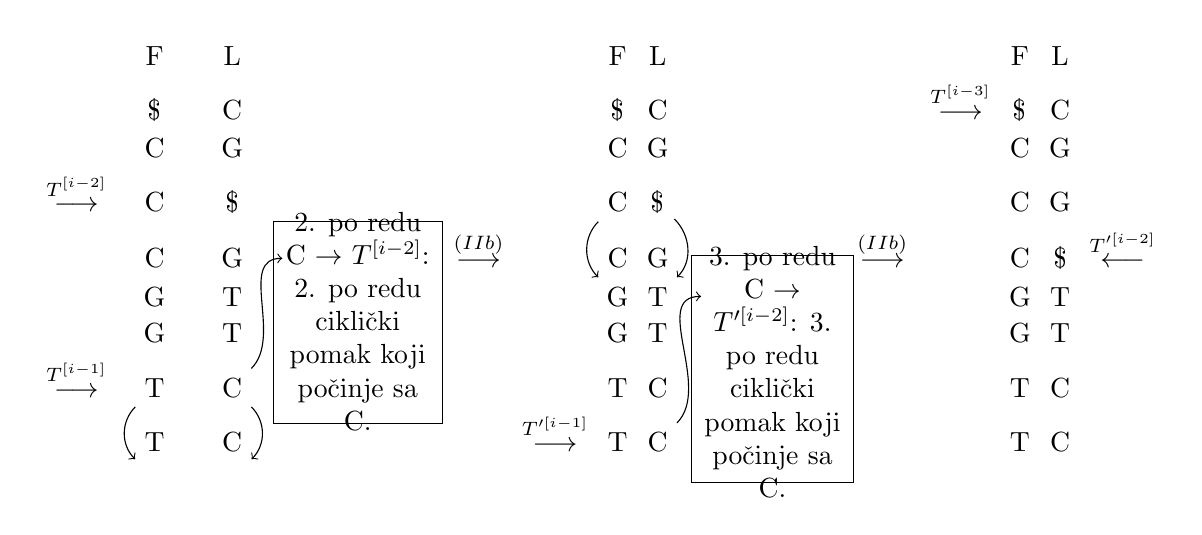
\begin{tikzpicture}
\matrix [matrix of nodes,row sep=-\pgflinewidth,name=table,column 4/.style={nodes={,minimum width=1.9cm}},column 9/.style={nodes={,minimum width=1.8cm}}](m)
{
	& F & L & [1ex] & [1ex] & & F & L & [2ex] & & & F & L & \\
	& \$ & C & & & & \$ & C & & & $\stackrel{T^{[i-3]}}{\longrightarrow}$ & \$ & C & \\
	& C & G & & & & C & G & & & & C & G & \\
	$\stackrel{T^{[i-2]}}{\longrightarrow}$& C & \$ & & & & C & \$  & & & & C & G & \\
	& C & G & \phantom{dank} & $\stackrel{(IIb)}{\longrightarrow}$ & & C & G & &$\stackrel{(IIb)}{\longrightarrow}$ & & C & \$ & $\stackrel{T'^{[i-2]}}{\longleftarrow}$ \\
	& G & T &  & & & G & T & \phantom{dank} & & & G & T & \\
	& G & T &  & & & G & T & \phantom{dank} & & & G & T & \\
	$\stackrel{T^{[i-1]}}{\longrightarrow}$& T & C & \phantom{dank} & & & T & C & \phantom{dank} & \phantom{dank} & & T & C & \\
	& T & C & \phantom{dank} & & $\stackrel{T'^{[i-1]}}{\longrightarrow}$ & T & C & \phantom{dank} & & & T & C & \\
	& \phantom{dank} & \phantom{dank} &   & &  &  &    & & &  &  & \\
};
\draw[->] (m-8-2) to [out=-135,in=135] (m-10-2);
\draw[->] (m-8-3) to [out=-45,in=45] (m-10-3);

\node[draw,fit=(m-5-4)(m-8-4)]{2. po redu C $\rightarrow$ $T^{[i-2]}$: 2. po redu ciklički pomak koji počinje sa C. };
\node[draw,fit=(m-6-9)(m-9-9)]{3. po redu C $\rightarrow$ $T'^{[i-2]}$: 3. po redu ciklički pomak koji počinje sa C. };

\draw[->] (m-4-8) to [out=-45,in=45] (m-6-8);
\draw[->] (m-4-7) to [out=-135,in=135] (m-6-7);

\draw[->] (m-8-3) to [out=45,in=180] (m-5-4);
\draw[->] (m-9-8) to [out=45,in=180] (m-6-9);

\end{tikzpicture}
\end{figure}
\normalsize
\subsection{Umetanje više od jednog znaka}
Umetanje prikazano u prethodnom poglavlju može se generalizirati za umetanje niza $S$ duljine $m$ na poziciju $i$ u $T$. Za $T'=T[0..i-1]S[0..m-1]T[i..n]$ gdje je $m>1$ koraci iz prethodnog poglavlja mogu se proširiti:
\begin{itemize}
	\item[(Ia)] Ciklički pomaci $T'^{[j]}$ gdje je $j>i+m$: ostaju nepromijenjeni.
	\item[(Ib)] Ciklički pomak $T'^{[i+m]}$: modifikacija $L=S_{m-1}$ umjesto $T_{i-1}$.
	\item[(IIa)] Ciklički pomaci $T'^{[j]}$ gdje je $i+1<j<i+m-1$:
	\begin{itemize}
		\item[] umetanje $F=S_{j-1}$ i $L=S_{j-i-1}$.
		\item[$T'^{[i]}$:] umetanje  $F=S_0$ i $L=T_{[i-1]}$
	\end{itemize}
	\item Ciklički pomaci $T'^{[j]}$ gdje je $j<i$Č isti algoritam kao i kod umetanja jednog znaka.
\end{itemize}
Kod umetanja više znakova pojavljuje se problem. U koraku (Ib) se briše $T_{i-1}$ i nakon svih umetanja potreban je na kraju korak (IIa). U koraku (IIa), sve vrijednosti koje koriste $rank_{T_{i-1}}$ izračunate prije zadnjeg umetanja mogu biti krive. Jednostavno rješenje ovog problema je da se kod računanja vrijednosti na koje utječe $rank_{T_{i-1}}$ izračunatoj vrijednosti doda $1$.
\subsection{Brisanje više od jednog znaka}
Briše se $m$ uzastopnih znakova u $T$, počevši od pozicije $i$. Dobiveni niz je $T'=T[0..i-1]T[i+m..n]$. Koraci se proširuju na sljedeći način:
\begin{itemize}
	\item[(Ia)] Ciklički pomaci $T'^{[j]}$ gdje je $j>i+m$: ostaju nepromijenjeni.
	\item[(Ib)] Ciklički pomak $T'^{[i+m]}$: modifikacija $L=T_{i-1}$ umjesto $T_{i+m-1}$.
	\item[(IIa)] Ciklički pomaci $T^{[j]}$ gdje je $i<j<i+m-1$:
	\begin{itemize}
		\item[] brisanje retka
		\item[] tijekom brisanja cikličkog pomaka, $T_{i-1}$ se pojavljuje dva puta u $L$. Potrebno je oduzeti $1$ od vrijednosti $rank_{T_{i-1}}$
	\end{itemize}
	\item Ciklički pomaci $T'^{[j]}$ gdje je $j<i$Č isti algoritam kao i kod umetanja jednog znaka.
\end{itemize}
\subsection{Zamjena više od jednog znaka}
Mijenja se $T[i..i+m-1]$ za $S[0..m-1]$. Dobiveni niz je $T'=T[0..i-1]S[0..m-1]T[i+m..n]$. Koraci se proširuju na sljedeći način:
\begin{itemize}
	\item[(Ia)] Ciklički pomaci $T'^{[j]}$ gdje je $j>i+m$: ostaju nepromijenjeni.
	\item[(Ib)] Ciklički pomak $T'^{[i+m]}$: modifikacija $L=S_{m-1}$ umjesto $T_{i+m-1}$.
	\item[(IIa)] Ciklički pomaci $T'^{[j]}$ gdje je $i+1<j<i+m-1$:
	\begin{itemize}
		\item[] zamjena $F=S_{j-i}$ i $L=S_{j-i-1}$
		\item[] pomaknuti redak na odgovarajuću poziciju.
		\item[$T'^{[i]}$] modifikacija $F=S_0$
	\end{itemize}
	\item Ciklički pomaci $T'^{[j]}$ gdje je $j<i$Č isti algoritam kao i kod umetanja jednog znaka.
\end{itemize}
\section{Testiranje i rezultati}
U testiranje je uključeno testiranje točnosti, testiranje vremena izvođenja i testiranje memorijskog zauzeća. Rezultati vremenskog i memorijskog testiranja prikazani su u tablici \ref{tablica:vremena}. Provedena je i usporedba vremena izvođenja za ponovnu izgradnju BWT-a i dodavanje i brisanje pomoću opisanog algoritma. Rezultati su prikazani u tablici \ref{tablica:usporedba}.
\subparagraph{}
Točnost je bila testirana koristeći UNIT testove. Podaci za usporedbu generirani su pomoću naivne implementacije BWT-a u Pythonu. Vremena izvođenja testirana su pomoću time.h biblioteke u kodu. Memorijsko zauzeće mjereno je alatom cgmemtime, dostupnom na https://github.com/isovic/cgmemtime.
\begin{table}[h]


\begin{tabular}{|m{7cm}|c|c| }
	\hline
	Opis testa i parametri & Vrijeme izvođenja [s] & Zauzeto memorije \\
	\hline
	građenje strukture, duljina 1031 & 0.003357 & 1MB \\
	\hline
	građenje strukture, duljina 5385 & 0.028451 & 1MB \\
	\hline
	građenje strukture, duljina 35970 & 0.176832 & 1MB \\
	\hline
	građenje strukture,  duljina 189561 & 1.214295 & 2MB \\
	\hline
	građenje strukture, duljina 2494862 & 21.097746 & 9MB \\
	\hline
	dodavanje od 512, u niz od 1032, na poziciji 512   & 0.001728 & 1MB \\
	\hline
	brisanje od 512, u nizu od 1032, na poziciji 500   & 0.001916 & 1MB \\
	\hline
	brisanje od 512, u nizu od 35970, na poziciji 10000   & 0.002748 & 2MB \\
	\hline
	dodavanje od 1413, u niz od 189561, na poziciju 10000   & 0.010186 & 2MB \\
	\hline
	brisanje od 42000, u nizu od 189561, na poziciji 20000   & 0.0203301 & 2MB \\
	\hline
	brisanje od 126183, u nizu od 700918, na poziciji 350000   & 0.738056 & 4MB \\
	\hline
	dodavanje od 126183, u niz od 700918, na poziciju 350000   & 0.902695 & 4MB \\
	\hline	
\end{tabular}
\caption{Vremena izvođenja i zauzeće memorije}
\label{tablica:vremena}
\end{table}
\begin{table}[h]
\begin{tabular}{|m{5cm}|c|c|}
	\hline
	Provedene operacije & Vrijeme za izgradnju BWT-a & Vrijeme ažuriranja \\
	\hline
	Dodavanje 4000 znakova na poziciju 4000 u niz od 35970 znakova & 0.157335 & 0.016616 \\
	\hline
	Brisanje 524 znaka na poziciju 500 u nizu od 3631 znakova & 0.013593 & 0.002038 \\
	\hline
\end{tabular}
\caption{Usporedba ponovne izgradnje i ažuriranja BWT-a}
\label{tablica:usporedba}
\end{table}

\section{Zaključak}
\dodajliteraturu{bazaLiterature}
\section{Sažetak}
\end{document}
